\section{Drive Box Assembly}

The drive box is an aluminum structure build to house the external belt drive system. It consists of four separate aluminum plates bolted together around the perimeter for modular assembly. Three of the plates are structural, while the fourth frontmost plate serves only a sealing purpose. There are five separate bearing housings protruding from the drive box and bolted to the structural plates: three in the front (the wheel shaft passes through two of them), and two in the back. The pivot is bolted through the back plate. The drive box is shown in Figures~\ref{fig:box_bld} and~\ref{fig:box_in}. Buna-N o-rings are installed between each separate component of the drive box to ensure proper sealing.

\begin{figure}[htbp]
\centering
\begin{minipage}{0.45\linewidth} \centering
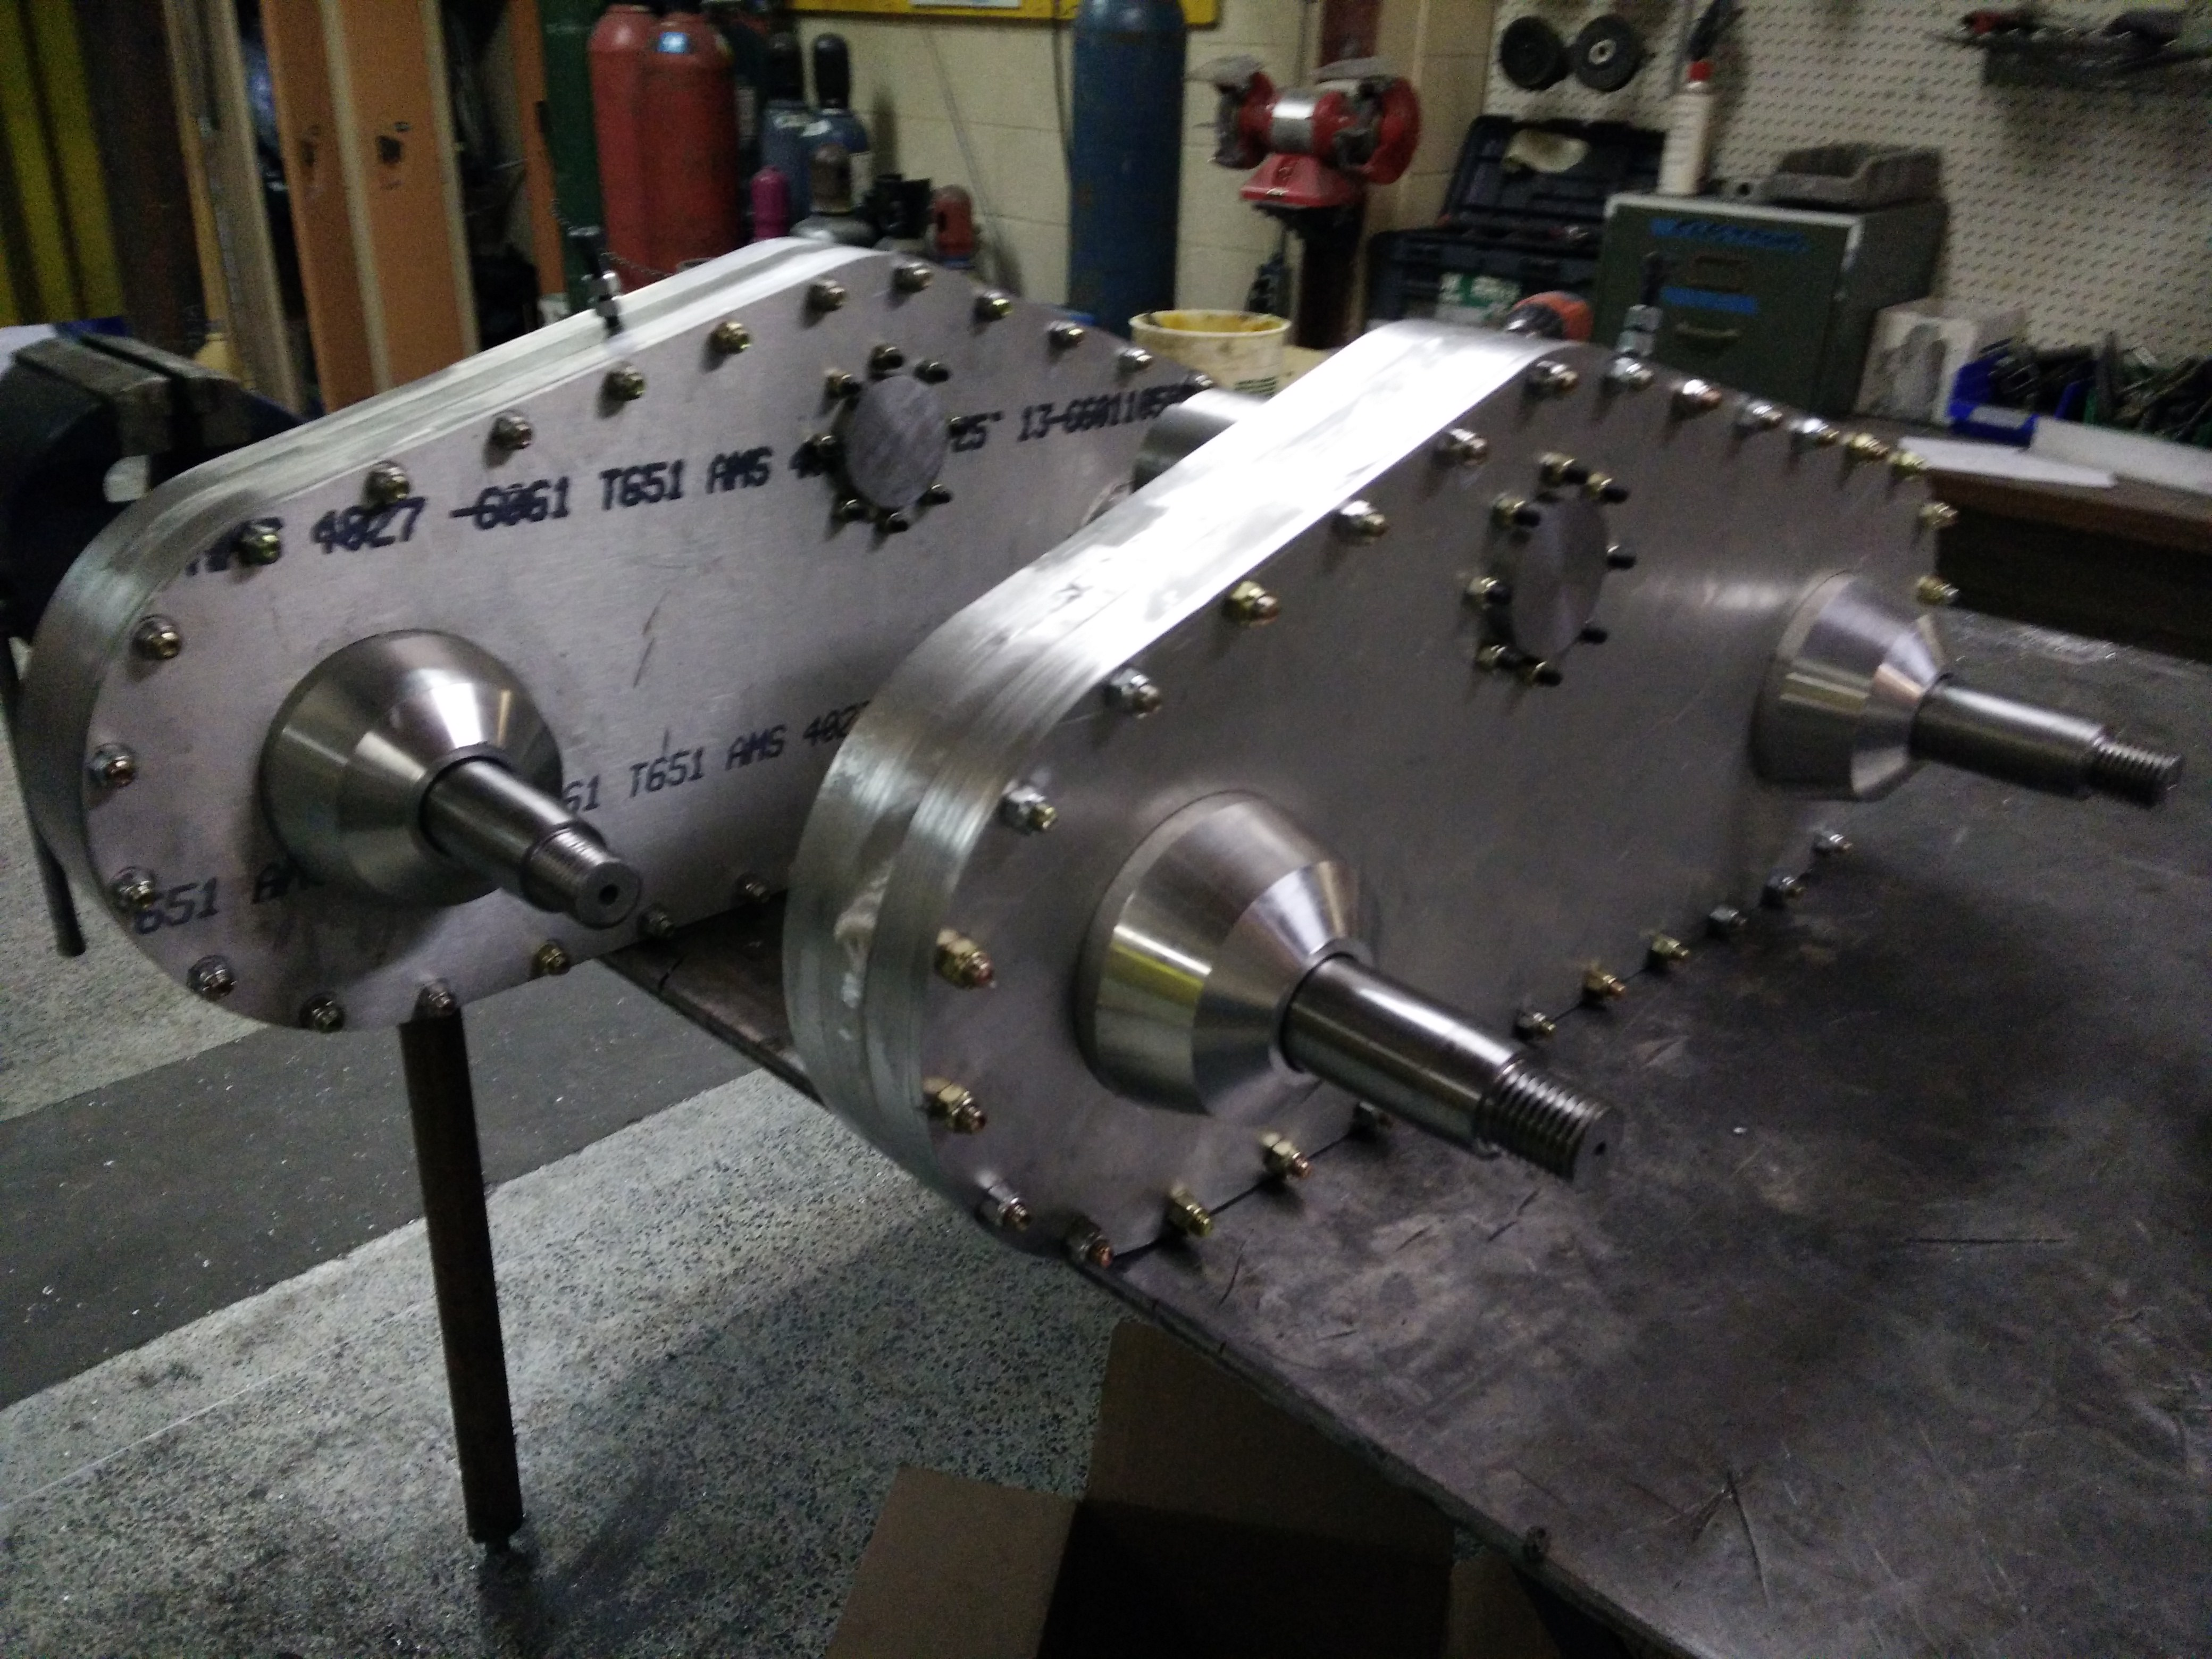
\includegraphics[height=0.22\textheight]{images/drive_box_assembly_NEW_bld}
\captionof{figure}[Completed Drive Boxes]{Two completed drive boxes before being mounted on the robot. One is the mirror image of the other.}
\label{fig:box_bld}
\end{minipage}
\hfill
\begin{minipage}{0.45\linewidth}
\centering
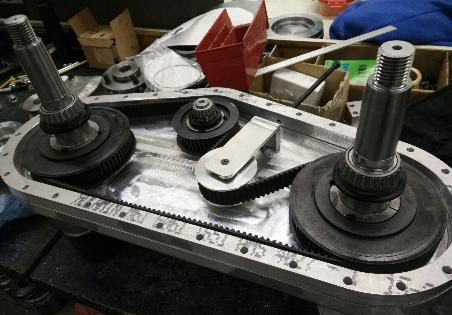
\includegraphics[height=0.22\textheight]{images/drive_box_open_bld}
\captionof{figure}[Interior of the Drive Boxes]{The drive box houses two wheel shaft assemblies, one drive shaft assembly, the belt, and tensioner.}
\label{fig:box_in}
\end{minipage}
\end{figure}

\subsection{Design Constraints}

The main constraints imposed on the drive box design are dimensional since the drive box design is constrained by the components in houses. It houses the belts, sprockets, bearing, seals, and tensioner. These components must also be laid out as defined by the shaft design software as presented in Section~\ref{SECTION LABEL FOR SHAFT}. %% TODO
Drive box dimension constraints are summarized in Table~\ref{tab:box_dim}. The drive box must be large enough to fit all the components, with additional clearance around the belt and sprocket for installation ease.

\begin{table}[htbp]
\centering
\caption{Gearbox dimension constraints}
\begin{tabular}{| lll |}\hline
Component & Dimension & Value \\ \hline
\multirow{2}{*}{Driving sprocket} & Diameter & 5  in \\
& Width & over 1.5 in \\
\multirow{2}{*}{Wheel sprocket} & Diameter & 7.6  in \\
& Width & over 1.5 in \\ \hline
\end{tabular}
\label{tab:box_dim}
\end{table}

Component drawings for the gearbox are given in Appendix~\ref{CITE APPENDIX}. Assembly drawings are also given with the bill of materials.

\subsection{Functional Requirements}

The drive boxes serve two main purposes: house the interior components from the environment and support the weight of the robot with negligible deflection. Therefore, the drive box must be adequately sealed to prevent entry of fluids and/or dust particles that can cause belts to slip. They must also be strong enough not to deflect under the weight of the robot, or under the high forces seen during skid steers. This requirement is important for the obvious reason, but it is of particular importance for a belt drive. Sprockets must not lie out of plane, as this puts point loads on the belt and decrease its life.

\subsection{Analysis and Design}

% TODO calcs, FEA, justify material selection, justify changes

\subsection{Belt Tensioner}

The belt tensioner is a custom-made, static, screw adjusted tensioner. The belt sits in an aluminum pulley. Sealed roller bearings are pressed into the pulley and the assembly is pressed onto a shaft that fits into a aluminum bracket. A screw threaded through the drive box centre plate presses against a thin steel plate mounted on top of the bracket to tension the belt. The assembly is shown in Figure~\ref{fig:box_in}. The brackets slides along slots milled out of the drive box plates.

\subsubsection{Design and Analysis}

The tensioner must withstand the loads applied by the tensioned belt. Therefore, an FEA analysis was conducted on the assembly. For the analysis, the top of the bracket was held fixed, and a load of 5600 N was applied to the shaft in a vertical upward direction. The results showed that the maximum displacement experienced by the tensioner was ${3.162*10^{-2}}$ mm and the maximum stress in 53.76 MPa, well below the yield strength of 1045 steel. These results were confirmed with deflection calculations in Matlab, yielding a deflection of ${4.1913*10^{-2}}$ mm. The results are shown in Figure~\ref{APPENDIX THIS} and~\ref{fig:REF THIS} in Appendix~\ref{fea}.


